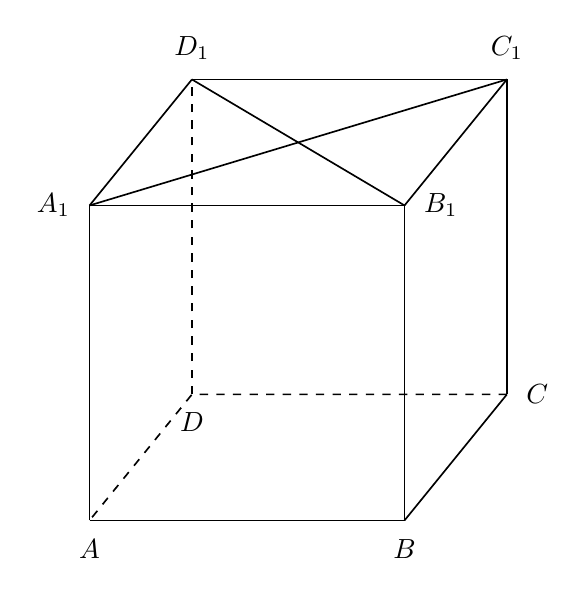
\begin{tikzpicture}[x=1cm,y=1cm,line width=0.6pt]
\coordinate (A) at (0,0);
\coordinate (B) at (4,0);
\coordinate (C) at (5.3,1.6);
\coordinate (D) at (1.3,1.6);
\coordinate (A1) at (0,4);
\coordinate (B1) at (4,4);
\coordinate (C1) at (5.3,5.6);
\coordinate (D1) at (1.3,5.6);
% bottom face
\draw[draw=black] (A) -- (B);
\draw[draw=black] (B) -- (C);
\draw[draw=black,dashed] (C) -- (D) -- (A);
% verticals
\draw[draw=black] (A) -- (A1);
\draw[draw=black] (B) -- (B1);
\draw[draw=black] (C) -- (C1);
\draw[draw=black,dashed] (D) -- (D1);
% top face
\draw[draw=black] (A1) -- (B1);
\draw[draw=black] (B1) -- (C1);
\draw[draw=black] (C1) -- (D1);
\draw[draw=black] (D1) -- (A1);
% top diagonals
\draw[draw=black] (D1) -- (B1);
\draw[draw=black] (A1) -- (C1);
% labels
\node[anchor=north,font=\normalsize] at ([yshift=-0.12cm]A) {$A$};
\node[anchor=north,font=\normalsize] at ([yshift=-0.12cm]B) {$B$};
\node[anchor=west,font=\normalsize] at ([xshift=0.12cm]C) {$C$};
\node[anchor=north,font=\normalsize] at ([yshift=-0.10cm]D) {$D$};
\node[anchor=east,font=\normalsize] at ([xshift=-0.12cm]A1) {$A_{1}$};
\node[anchor=west,font=\normalsize] at ([xshift=0.12cm]B1) {$B_{1}$};
\node[anchor=south,font=\normalsize] at ([yshift=0.12cm]C1) {$C_{1}$};
\node[anchor=south,font=\normalsize] at ([yshift=0.12cm]D1) {$D_{1}$};
\end{tikzpicture}